%!TEX root = ../../prace.tex


\appendix
\chapwithtoc{Přílohy}

\renewcommand{\thesection}{\Alph{section}}

\section{Struktura souborů přílohy}
Struktura vypadá následovně:
\begin{itemize}
	\item \textit{Build} -- tato složka obsahuje výslednou zkompilovanou hru, kterou je možné spustit.
	\item \textit{Source} -- v~této složce se nachází zdrojové soubory hry.
	\item \textit{Survey} -- pod touto složkou je možné nalézt soubor dotazníku se získanými odpověďmi.
\end{itemize}



\section{Grafy k~dotazníku}
\label{sec:survey}


Níže je možné se podívat na grafy zpracované stránkou Google Forms. U~sloupcových grafů byla otázka zodpovězena na škále od 1 do 10. Krajní hodnoty, které byly v~dotazníku nabídnuty, jsou vepsány v~popisku obrázku.

\begin{figure}[!ht]\centering
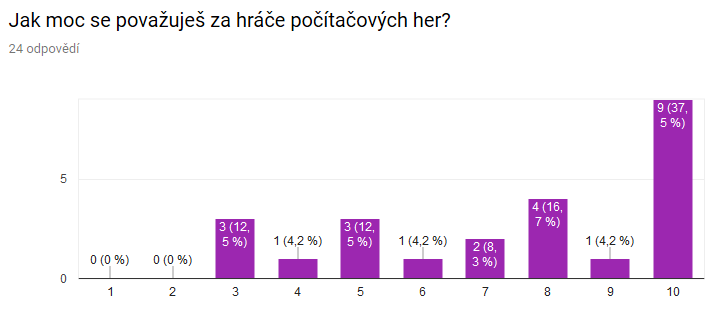
\includegraphics[ width=110mm]{../img/survey/q1}
\caption{Vůbec hry nehraji -- Hraji každý den}
\label{fig:q1}
\end{figure}
\FloatBarrier


\begin{figure}[!ht]\centering
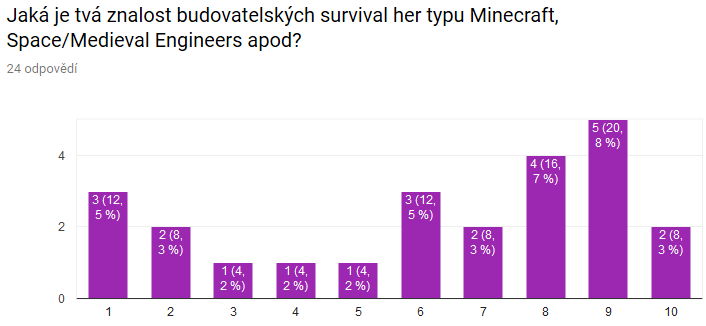
\includegraphics[ width=110mm]{../img/survey/q2}
\caption{Vůbec to neznám -- Znám je velice dobře}
\label{fig:q2}
\end{figure}
\FloatBarrier


\begin{figure}[!ht]\centering
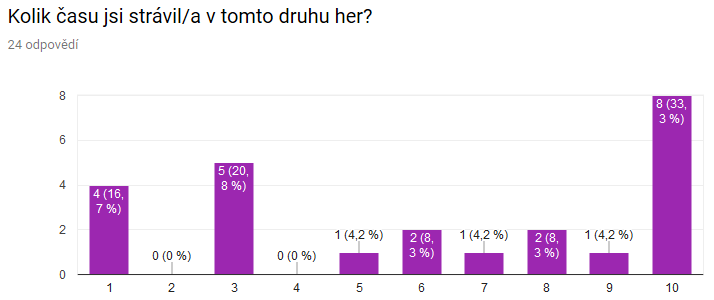
\includegraphics[ width=110mm]{../img/survey/q3}
\caption{Velice málo (max. 1 hodinu) -- Hodně (100 a~více hodin)}
\label{fig:q3}
\end{figure}
\FloatBarrier


\begin{figure}[!ht]\centering
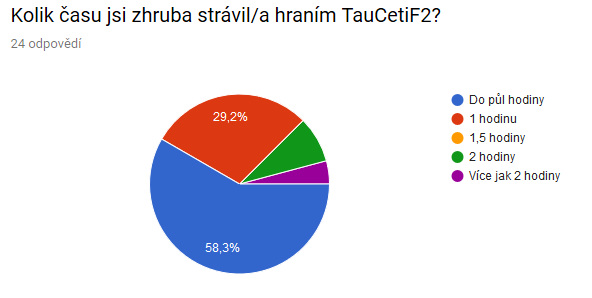
\includegraphics[ width=110mm]{../img/survey/q4}
\caption{Otázka 4}
\label{fig:q4}
\end{figure}
\FloatBarrier


\begin{figure}[!ht]\centering
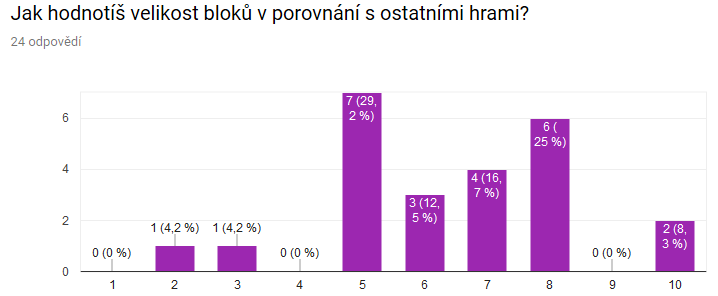
\includegraphics[ width=110mm]{../img/survey/q5}
\caption{Příliš malé -- Dostatečně velké}
\label{fig:q5}
\end{figure}
\FloatBarrier


\begin{figure}[!ht]\centering
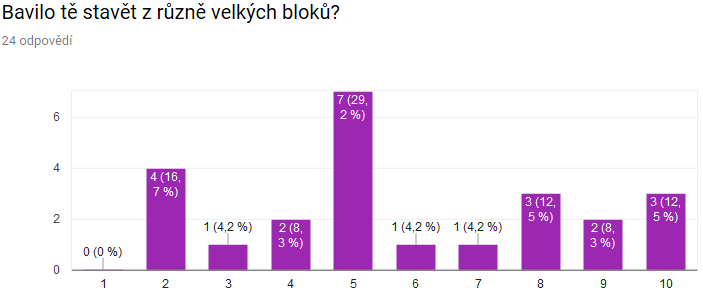
\includegraphics[ width=110mm]{../img/survey/q6}
\caption{Stavění bylo oproti jiným hrám nepříjemné -- Stavění mě oproti jiným hrám opravdu bavilo}
\label{fig:q6}
\end{figure}
\FloatBarrier


\begin{figure}[!ht]\centering
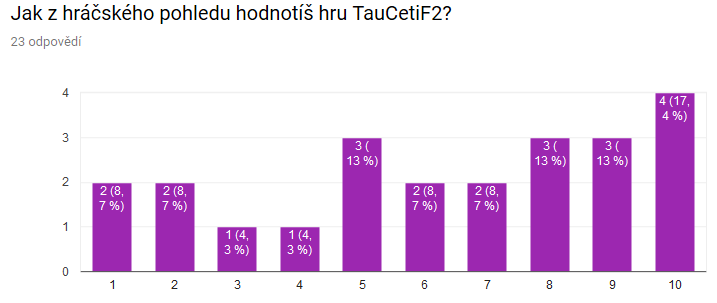
\includegraphics[ width=110mm]{../img/survey/q7}
\caption{Velice nepovedená, nikdy se k~ní nevrátím -- Zdařilá, rád/a bych si v~budoucnu dokončenou hru zahrál/a}
\label{fig:q7}
\end{figure}
\FloatBarrier


\newpage

\section{Struktura souboru uložené hry}
\label{sec:saveGame}
Základní struktura binárního souboru uložené hry je níže. Datové typy odpovídají datovým typům \UEu{} a~vlastním definovaným typům. Ty popíšeme v~následujících tabulkách. Vzhledem k~použití dědičnosti u~některých vlastních datových typů musíme přistoupit k~zápisu \TT{[název datového typu předka]} bez uvedení názvu vlastnosti. Tím dáváme najevo fakt, že daná struktura navíc obsahuje na dané pozici všechny datové položky daného předka. Dále u~některých vlastností využíváme podmínek. Pokud taková podmínka není splněna, data se v~binárním souboru vůbec neobjeví.

\begin{code}
FString                                     SaveName
FDateTime                                   SavedDate
FTimespan                                   PlayedTime
bool                                        IsQuickSave
uint8                                       MinBoxSize
float                                       CurrentTime
FVector                                     PlayerPosition
FRotator                                    PlayerRotation
FRotator                                    PlayerCameraRotation
bool                                        PlayerUseFPSCamera
TArray<FBlockInfo>                          usedBlocks
TArray<FInventoryBuildableBlockInfo>        buildableBlocks
TArray<FInventoryBuildableItemBlockInfo>    inventoryBuildableBlocks
FInventoryTags                              inventoryTags
int32                                       InventoryCurrentIndex
FOxygenComponentInfo                        PlayerOxygenComponent
FElectricityComponentInfo                   PlayerElectricityComponent
float                                       PlayerHealth
bool                                        IsCreativeMode
FWeatherState                               weatherState
\end{code}



\subsubsection{FBlockInfo}

\begin{code}
[FBlockBaseInfo]
FVector                                     Location
FRotator                                    Rotation
float                                       Health
TMap<FString, FString>                      BlockSpecificData
bool                                        HasRelationshipData
if (HasRelationshipData)
    FBlockWithRelationshipInfo              RelationshipInfo
\end{code}

\newpage


\subsubsection{FBlockWithRelationshipInfo}
\begin{code}
FGuid                                       ID
TArray<FRelationshipInfo>                   Relationships
\end{code}

\subsubsection{FRelationshipInfo}
\begin{code}
FGuid                                       TargetID
uint8                                       RelationshipType
\end{code}


\subsubsection{FBlockBaseInfo}
\begin{code}
int32                                       ID
FVector                                     Scale
FString                                     Name
TMap<FString, int32>                        AdditionalFlags
bool                                        HasOxygenData
if (HasOxygenData)
    FOxygenComponentInfo                    OxygenInfo
bool                                        HasElectricityData
if (HasElectricityData)
    FElectricityComponentInfo               ElectricityInfo
\end{code}





\subsubsection{FOxygenComponentInfo}
\begin{code}
float                                       CurrentObjectOxygen
\end{code}


\subsubsection{FElectricityComponentInfo}
\begin{code}
float                                       CurrentObjectEnergy
bool                                        HasPoweredBlockInfo
if (HasPoweredBlockInfo)
    FPoweredBlockInfo                       PoweredBlockInfo
\end{code}

\subsubsection{FPoweredBlockInfo}
\begin{code}
bool                                        IsOn
bool                                        AutoregulatePower
float                                       PowerConsumptionPercent
\end{code}



\subsubsection{FInventoryBuildableBlockInfo, FInventoryBuildableItemBlockInfo}
\begin{code}
TArray<FString>                             Tags
\end{code}

\newpage


\subsubsection{FInventoryTags}
\begin{code}
int32                                       CurrentActiveIndex
TArray<FInventoryTagGroup>                  InventoryGroupList
\end{code}

\subsubsection{FInventoryTagGroup}
\begin{code}
FString                                     GroupName
bool                                        IsGroupEnabled
uint8                                       GroupType
TArray<FTagGroup>                           GroupList
\end{code}

\subsubsection{FTagGroup}
\begin{code}
FString                                     GroupName
TArray<FString>                             Tags
bool                                        LetVisibleAll
\end{code}

\subsubsection{FWeatherState}
\begin{code}
int32                                       CurrentDefinitionID
bool                                        IsInWeatherChange
bool                                        ApplyDamage
float                                       CurrentWaitingTime
float                                       TargetWaitingTime
float                                       BaseWeatherIntensity
float                                       CurrentWeatherIntensity
float                                       TargetWeatherIntensity
float                                       BaseCloudOpacity
float                                       CurrentCloudOpacity
float                                       TargetCloudOpacity
float                                       HitpointsCounter
float                                       PlayerHitpointCounter
float                                       EaseIn
float                                       EaseOut
uint8                                       StormState
\end{code}